\documentclass[11pt,a4paper]{article}
\usepackage[margin=2.4cm]{geometry}
\usepackage[T1]{fontenc}
\usepackage[utf8]{inputenc}
\usepackage{lmodern}
\usepackage{microtype}
\usepackage{graphicx}
\usepackage{booktabs}
\usepackage{amsmath}
\usepackage{caption}
\usepackage{placeins}
\usepackage{xurl}
\usepackage[hidelinks]{hyperref}
\graphicspath{{figures/}}
\setlength{\parindent}{0pt}
\setlength{\parskip}{0.6em}
\captionsetup{font=small,labelfont=bf}
\newcommand{\Fa}{\textit{F.~aquilonia}}
\newcommand{\Fp}{\textit{F.~polyctena}}

\title{Founder LD in the neutral simulations:\\ current set-up versus empirical parents, and a mosaic alternative}
\author{Note for Beatriz (from Petri; analyses run with Claude)}
\date{\today}

\begin{document}
\maketitle

\section*{Summary}
\begin{itemize}
  \item The LD among the simulated parents (the founders) does not match the LD among the empirical parents. Founder LD is \emph{binary}: SNPs in the same \path{min_r2 = 0.2} cluster are in perfect LD ($r^2=1.000$), SNPs in different clusters are independent ($r^2\approx0.07$, the sampling floor for 15 individuals). Empirical parental LD is graded and intermediate. Averaged by distance, simulated short-range LD is two to three times too high and extends to 0.2--1~cM (Figures~\ref{fig:decay}, \ref{fig:close}).
  \item This matters downstream: in the current replicates, hybrid populations show far higher within-population LD and far longer shared ancestry patterns than the empirical hybrids, and part of this is likely inherited from the founders (Figure~\ref{fig:hybrid}).
  \item A simple alternative that needs no phasing --- building founders as \emph{genotype mosaics} of the 15 empirical parents per species --- reproduces the empirical LD decay, the graded LD of close pairs, allele frequencies and heterozygosity. Both tested switch rates (0.5 and 1 per cM) pass an acceptance test that the current founders fail. We recommend 1 switch per cM.
  \item Generator, acceptance test and figure scripts are in \path{formica_hybrid/sim_founder_fix/}. The founder files are per-chromosome VCFs that SLiM reads directly with \path{readHaplosomesFromVCF}.
  \item We also recommend adding about 14,100 near-neutral SNPs (parental diagnostic index $\leq-90$) to the simulated panel as a calibration anchor (Section~\ref{sec:anchor}); the generator has an option for this.
  \item This is separate from, and in addition to, the founder-frequency indexing bug in \path{AIMs_for_SLiM.R} (\path{NOTE_for_Beatriz.md}). Mosaic founders copy real genotypes SNP by SNP, so they do not use the AIMs probability files at all.
\end{itemize}

\section{What was compared}

LD was measured within each parental species as the genotype correlation $r^2$ between the 20,807 representative SNPs of the DI25 LD units used in the empirical analyses (\path{module_allele_specific_sorting}), counting only SNPs polymorphic in that species and data set. Pairs were grouped by genetic distance on the recombination map (pairs with identical interpolated map positions, i.e.\ undefined genetic distance, excluded), with all cross-chromosome pairs as an ``unlinked'' class. Pairs less than 5~kb apart were also split by whether both SNPs fall in the same simulation LD cluster (\path{group_info_new.rds}), because the current founder set-up assigns founder alleles cluster by cluster. Every data set was evaluated on 15 individuals per species, the empirical sample size, so that all share the same finite-sample floor ($E[r^2]\approx1/14\approx0.07$ for unlinked pairs). Haploid individuals were coded 0/2, so that their correlation is the gametic $r$.

Data sets: the 15 + 15 empirical reference parents; the 15 + 15 \path{aq_}/\path{pol_} parents of 20 existing replicates (\path{diem_outs_demo}, i.e.\ the founders sampled into each bootstrap); and ten random sets of 15 + 15 individuals drawn from mosaic founder pools (50 males + 50 queens) generated at 0.5 and 1 switch per cM.

\section{Current founders}

\begin{figure}[htbp]
  \centering
  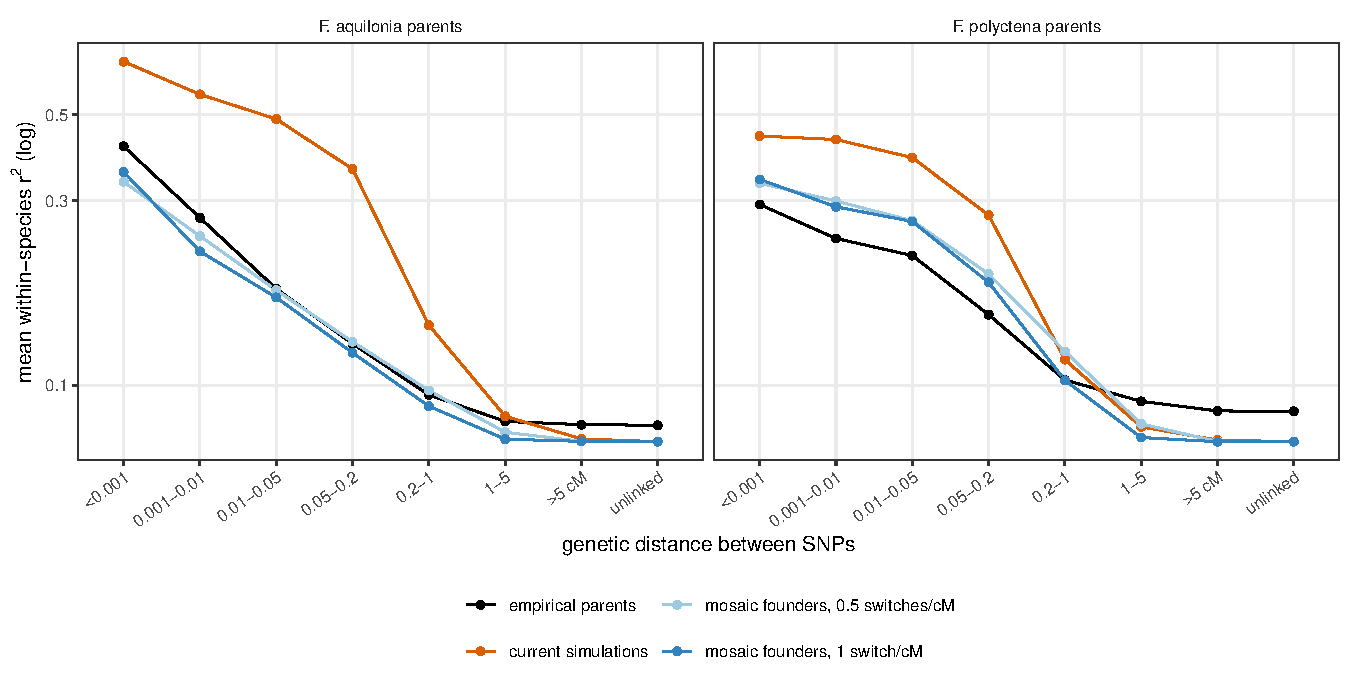
\includegraphics[width=\textwidth]{fig1_decay.pdf}
  \caption{Within-species LD of the parents by genetic distance: empirical parents (black), current simulated parents (orange; mean over 20 replicates) and mosaic founders at two switch rates (blue; mean over 10 sets of 15 individuals). $n=15$ in every case.}
  \label{fig:decay}
\end{figure}

\begin{figure}[htbp]
  \centering
  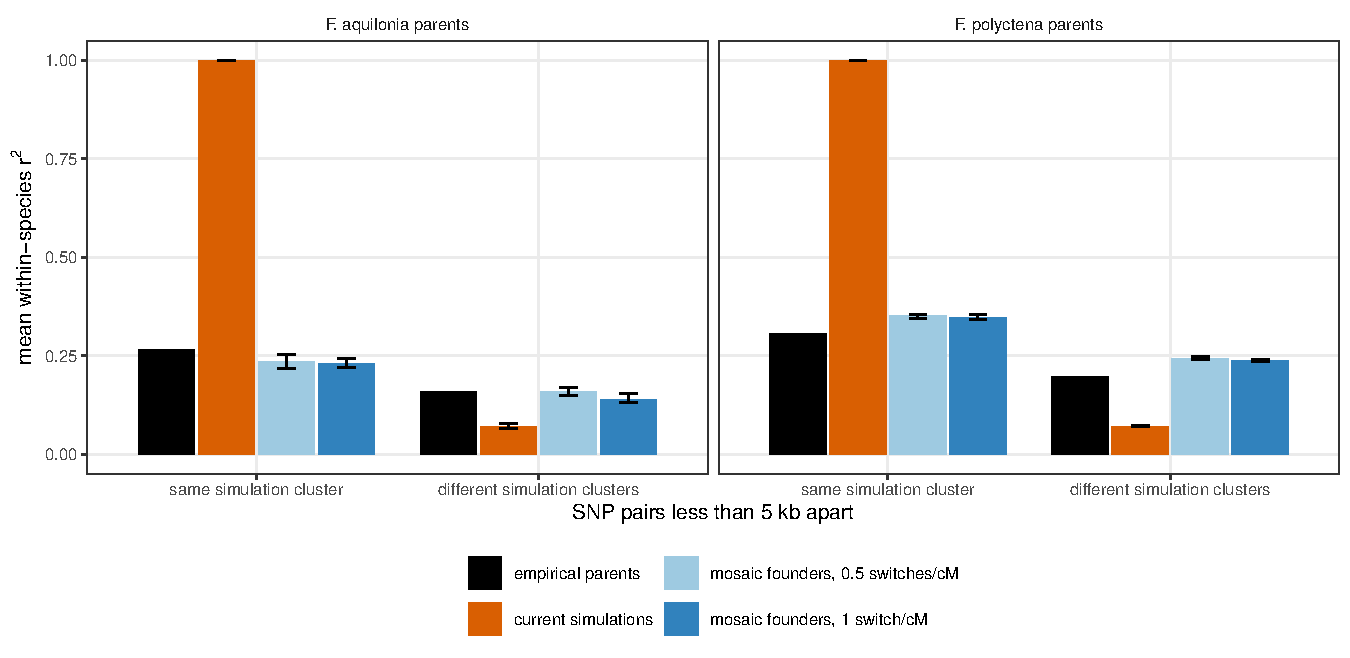
\includegraphics[width=\textwidth]{fig2_close_pairs.pdf}
  \caption{LD between SNPs less than 5~kb apart, split by whether both SNPs lie in the same simulation LD cluster. Error bars: range over replicates / sets.}
  \label{fig:close}
\end{figure}

Three differences stand out (Table~\ref{tab:numbers}):
\begin{enumerate}
  \item \textbf{Binary LD.} Close pairs in the same simulation cluster have $r^2=1.000$ in every replicate; close pairs in different clusters have $r^2=0.071$, the level of unrelated SNPs. In the empirical parents the same pairs have $r^2=0.27$--0.31 and 0.16--0.20. This is the direct consequence of drawing which founder haplosomes carry the allele once per cluster: all SNPs of a cluster are then carried by exactly the same founders, and neighbouring clusters are drawn independently. Including more loosely correlated SNPs in the clusters does not compensate for the independence between clusters; it enlarges the sets of SNPs in perfect LD. About 44\% of unit pairs less than 5~kb apart fall inside one simulation cluster.
  \item \textbf{Too much LD over too long a distance.} Averaged by distance, simulated $r^2$ is 0.62 vs 0.21 (\Fa) and 0.51 vs 0.25 (\Fp) within 5~kb, and 0.36 vs 0.13 at 0.05--0.2~cM. LD reaches background only at 1--5~cM. Conversely, empirical parents sit slightly above the floor even when unlinked (0.079--0.086 vs 0.071), probably because they were sampled from several localities.
  \item \textbf{Ploidy and heterozygosity.} All simulated \Fa\ parents are haploid (no heterozygotes): they are the founder males. The empirical parents are diploid workers (heterozygosity 0.055). Simulated \Fp\ parents are twice as heterozygous as the empirical ones (0.27 vs 0.12), consistent with the fixation levels (fractions of homozygous parents) being used as allele frequencies.
\end{enumerate}

\begin{table}[htbp]
\centering
\small
\caption{Mean within-species $r^2$ ($n=15$) and sample summaries. Mosaic founders: pools of 50 haploid \Fa\ males and 50 diploid \Fp\ queens, mean over 10 random sets of 15.}
\label{tab:numbers}
\resizebox{\textwidth}{!}{\begin{tabular}{llrrrr}
\toprule
Species & Class & Empirical & Current & Mosaic 0.5/cM & Mosaic 1/cM \\
\midrule
\Fa & $<5$~kb, same simulation cluster & 0.267 & 1.000 & 0.236 & 0.230 \\
    & $<5$~kb, different clusters & 0.160 & 0.071 & 0.158 & 0.140 \\
    & 0.001--0.01~cM & 0.271 & 0.565 & 0.243 & 0.222 \\
    & 0.05--0.2~cM & 0.128 & 0.362 & 0.130 & 0.121 \\
    & 0.2--1~cM & 0.094 & 0.143 & 0.097 & 0.088 \\
    & 1--5~cM & 0.081 & 0.083 & 0.076 & 0.073 \\
    & unlinked & 0.079 & 0.071 & 0.071 & 0.071 \\
    & heterozygosity & 0.055 & 0 (haploid) & 0 (haploid) & 0 (haploid) \\
\midrule
\Fp & $<5$~kb, same simulation cluster & 0.307 & 1.000 & 0.352 & 0.348 \\
    & $<5$~kb, different clusters & 0.198 & 0.071 & 0.244 & 0.238 \\
    & 0.001--0.01~cM & 0.240 & 0.432 & 0.299 & 0.289 \\
    & 0.05--0.2~cM & 0.152 & 0.275 & 0.194 & 0.184 \\
    & 0.2--1~cM & 0.103 & 0.116 & 0.122 & 0.103 \\
    & 1--5~cM & 0.091 & 0.078 & 0.079 & 0.073 \\
    & unlinked & 0.086 & 0.071 & 0.072 & 0.071 \\
    & heterozygosity & 0.125 & 0.266 & 0.124 & 0.124 \\
\midrule
\multicolumn{2}{l}{Acceptance test (below)} & --- & FAIL (7 of 10) & PASS & PASS \\
\bottomrule
\end{tabular}}
\end{table}

\section{Why it matters for the hybrid-population comparisons}

\begin{figure}[htbp]
  \centering
  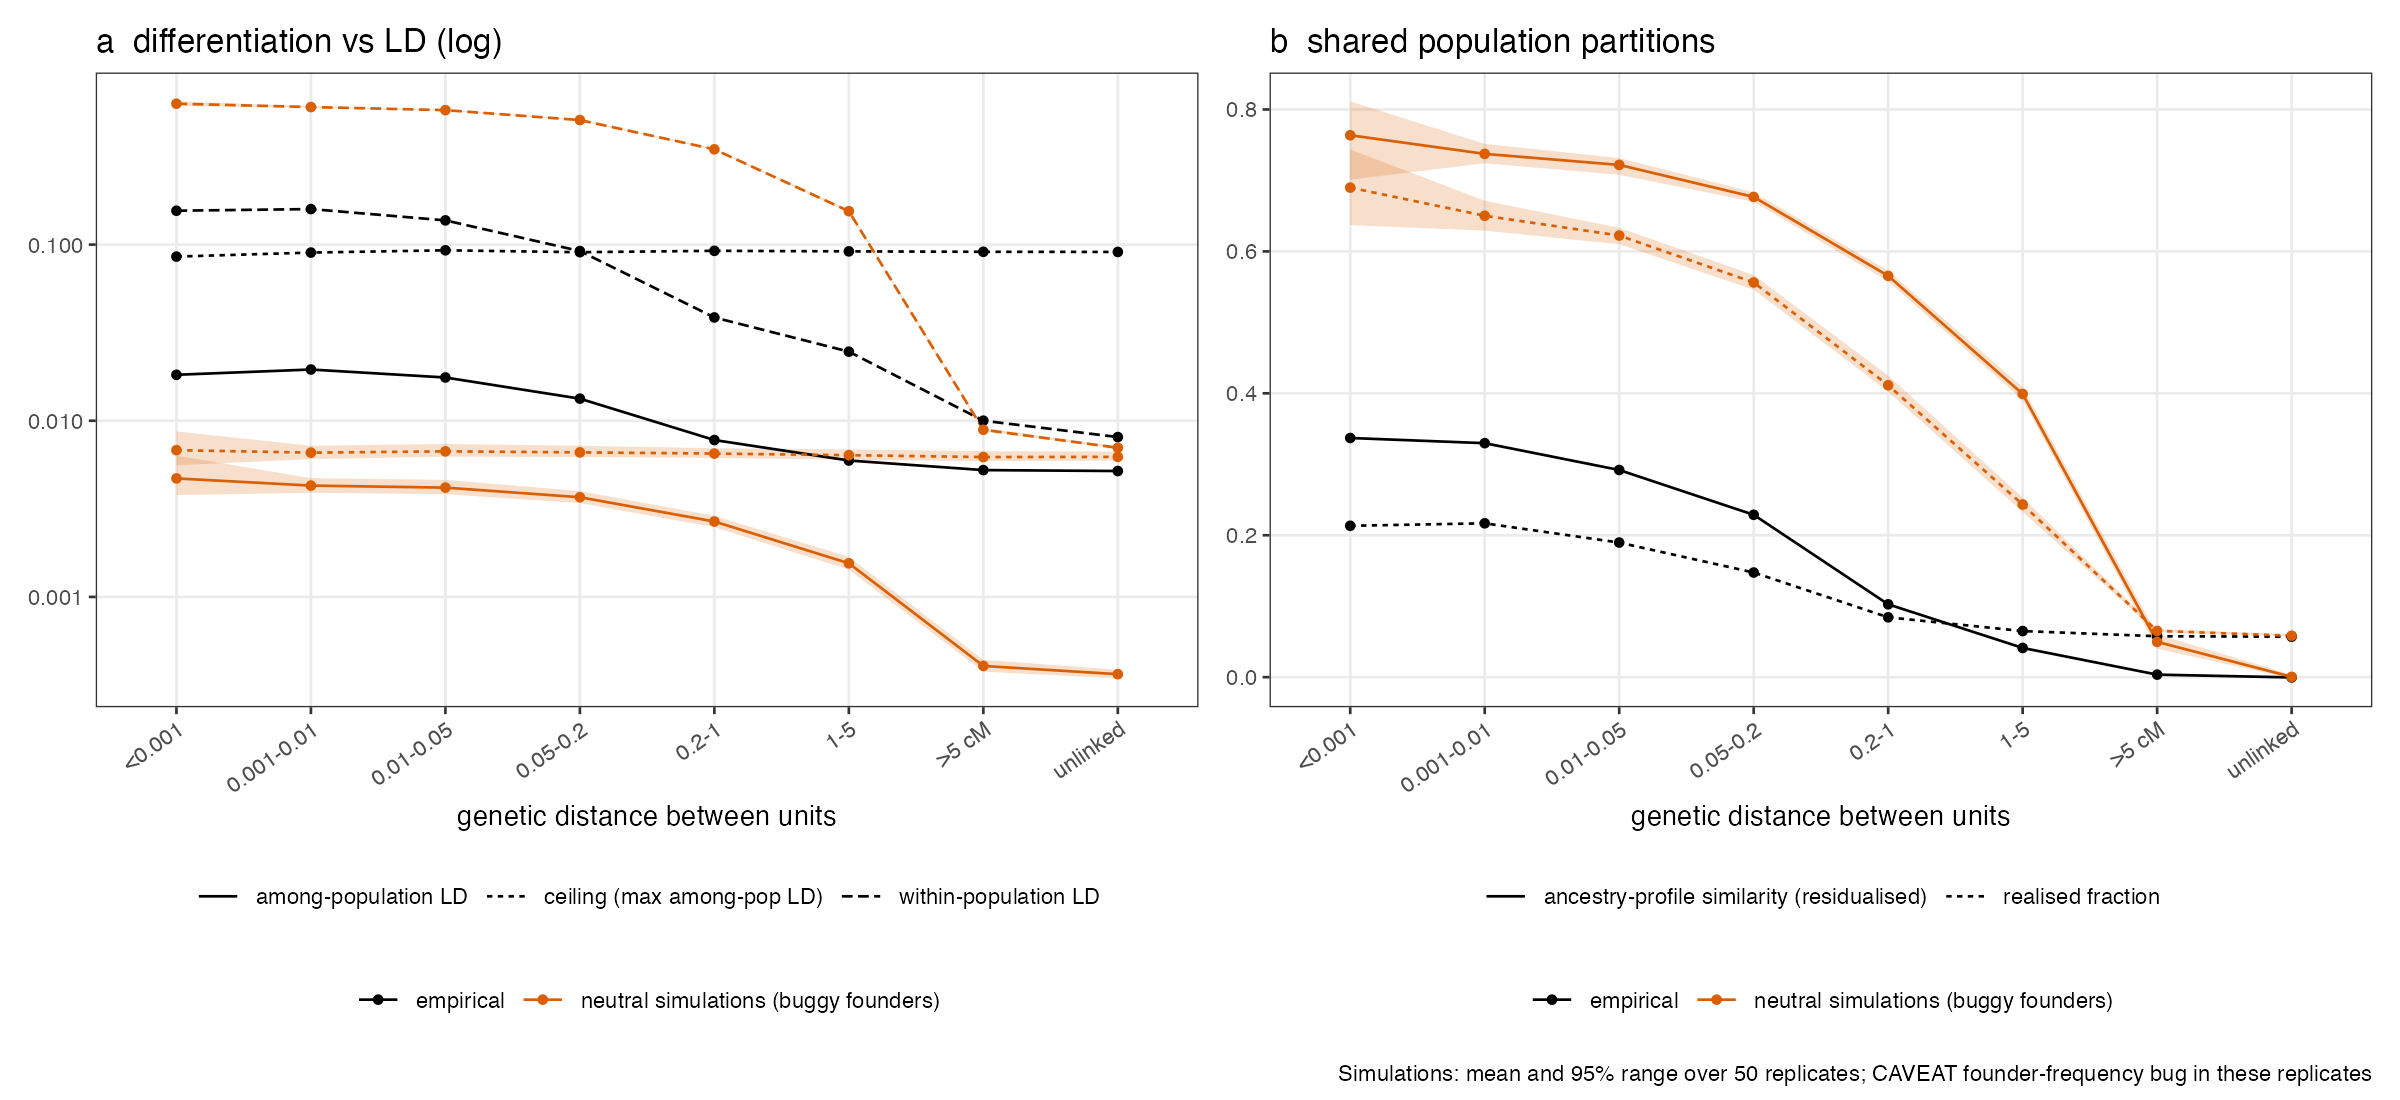
\includegraphics[width=\textwidth]{fig3_hybrid_preview.png}
  \caption{Preview with the \emph{current} replicates (50; founder-frequency bug and founder LD as described): among-population LD and its ceiling, within-population LD (\textbf{a}), and the fraction of the among-population LD ceiling realised and ancestry-profile similarity among hybrid populations (\textbf{b}), by genetic distance between LD units. Black: empirical hybrids; orange: simulations.}
  \label{fig:hybrid}
\end{figure}

In the empirical hybrids, ancestry-informative loci are strongly differentiated, but different loci distinguish different populations and shared ancestry patterns decay within about 1~cM. In the current simulations the opposite holds: differentiation is weak, but what exists is shared over long distances, and within-population LD among hybrids is about four times the empirical level at short range, staying high to several cM (Figure~\ref{fig:hybrid}). Founders whose LD is perfect within clusters and decays only beyond 0.2--1~cM would produce exactly such long shared blocks, and 130 generations of recombination erode short-range LD only slowly. The hybrid-level comparison is therefore not interpretable until the founders' LD matches the empirical parents.

\section{Mosaic founders}

\paragraph{Recipe.} Each founder is built chromosome by chromosome. Start with a random donor among the 15 empirical parents of its species and copy the donor's genotypes; switch to a new random donor at breakpoints placed along the genetic map as a Poisson process with $\lambda$ switches per cM. Missing donor genotypes are filled, per site, from a random donor of the same species. For haploid \Fa\ males one allele is taken from the copied diploid genotype (homozygotes as is; heterozygotes at random). For diploid \Fp\ queens the copied genotype is used and heterozygous sites are split at random between the two haplosomes. All 51,612 DI25 SNPs are written.

\paragraph{Results.} Mosaic founders reproduce the empirical decay of LD with genetic distance at both switch rates (Figure~\ref{fig:decay}) and, unlike the current founders, give graded LD between close SNPs in the same and in different simulation clusters (Figure~\ref{fig:close}). For \Fa\ the match is close at all distances. For \Fp\ short-range $r^2$ is about 0.04--0.05 too high. This residual excess is expected with only 15 donors: at any position, a sample of founders copies a few of the same donors, so the empirical sample's own noise is copied into the founders as if it were LD. Polyctena heterozygosity matches the empirical value (0.124 vs 0.125). The switch rate trades LD fidelity against new haplotype diversity. At 1 switch per cM, a chromosome of 140--350~cM is copied from 140--350 donor segments averaging 1~cM (roughly 45~kb at the genome-median 22~cM/Mb); this rate matched the 0.2--1~cM class best, so we recommend $\lambda=1$.

\paragraph{Side effects to be aware of.}
\begin{itemize}
  \item Founders are built from a finite set of 15 donors per species, so the founder pool carries less haplotype diversity than a real population sample would. Single-locus founding variance is unchanged (each founder segment is a random draw from the donor sample), but multilocus diversity is limited.
  \item Haploid males lose polymorphism at sites where the donors are mostly heterozygous; in samples of 15 males, about 6,900 of the evaluation SNPs are polymorphic, versus 9,900 in the 15 diploid empirical parents.
  \item Phase among neighbouring heterozygous sites is random. Heterozygosity at DI25 sites is low (0.05--0.12), so few pairs are affected.
\end{itemize}

\section{Calibration anchor: near-neutral markers}
\label{sec:anchor}

The current simulations contain only the 51,612 ancestry-informative DI25 SNPs, so the amount of drift they produce is calibrated only indirectly. Near-neutral SNPs, where the parents barely differ (diagnostic index $\leq-90$), provide a direct anchor: drift and demography act on all loci alike, but ancestry sorting cannot act where the parents do not differ. Empirically these loci are only weakly differentiated among the hybrid populations ($F_{ST}\approx0.05$, mean Nei-type $G=0.044$, versus 0.30 at DI25 units). A neutral model that reproduces this background at near-neutral loci, but not the differentiation at ancestry-informative loci, isolates an ancestry-specific excess; an earlier attempt of Petri's to build such a null over-drifted at these loci ($F_{ST}\approx0.14$), which would have made the comparison too lenient.

Mosaic founders make this straightforward, because they copy whatever markers they are given. With \texttt{PANEL = "DI25+neutral"} the generator adds the 14,093 SNPs with diagnostic index $\leq-90$ and pooled parental minor-allele frequency $\geq0.15$ (65,705 SNPs in total; the near-neutral IDs are written to \path{neutral_markers.txt}). In a test pool, founder allele frequencies at these SNPs reproduced the empirical parental frequencies (\Fp: $r=0.98$, mean absolute difference 0.023; \Fa: $r=0.83$, 0.056, as expected from sampling one allele per haploid male in a pool of 50). For 26 near-neutral SNPs no \Fa\ parent had an observed genotype; the generator then writes allele 0 for all \Fa\ founders at those sites.

Empirically, the near-neutral loci are also informative about the \emph{structure} of differentiation, not only its level: relative to their own (much lower) differentiation, they share their population pattern more between chromosomes and less over linkage distances than the ancestry-informative loci, and within-population LD between them extends to about 0.05~cM rather than 1--5~cM. Simulations should reproduce these near-neutral patterns too.

\section{How to use}

From the \path{formica_hybrid} repository root:
\begin{verbatim}
# one founder pool per SLiM run (vary SEED with the run);
# add the near-neutral calibration markers with PANEL = DI25+neutral
Rscript sim_founder_fix/make_mosaic_founders.R <OUT_DIR> 1 50 50 <SEED> \
    DI25+neutral

# acceptance test on a founder pool (10 random sets of 15 + 15)
Rscript sim_founder_fix/check_parent_ld.R vcf <OUT_DIR> 10

# acceptance test on finished DIEM bootstrap outputs (their aq_/pol_ parents)
Rscript sim_founder_fix/check_parent_ld.R bed \
    data/diem_outs_demo/diem_boot*_output.bed
\end{verbatim}
The VCFs use the same format as Petri's earlier attempt to seed the simulations with real, phased parental haplotypes (SLiM script \path{SpecIAnt_rufa_neutral_realfounders.slim}): \path{founders_ch<id>.vcf}, columns \path{aq_hapNN} (haploid, 0/1) then \path{pol_femNN} (phased diploid), \texttt{POS} = genome position, allele 1 = the coded allele of \path{module_di25/data/di25_inputs.rds}. The founder block of \path{SpecIAnt_rufa_genome_LDclusters_demo_server.slim} would be replaced by the founder-loading block of that earlier script, which reads the files with \path{readHaplosomesFromVCF} (p1 males, p2 queens; one read per chromosome so that both species share one mutation per site). The SLiM side has not been changed or tested here.

\paragraph{Acceptance test} (\path{check_parent_ld.R}; thresholds pragmatic): (1) no LD class has mean $r^2\geq0.9$; (2) close pairs in different simulation clusters keep at least 75\% of the empirical $r^2$; (3) close pairs in the same simulation cluster are within $\pm0.10$ of the empirical $r^2$; (4) the 0.2--1~cM and 1--5~cM classes are within $\pm0.03$ of the empirical values. Current founders fail checks 1--3 for both species and check 4 at 0.2--1~cM for \Fa; both mosaic pools pass all checks.

\end{document}
